\documentclass[a4paper]{article}

%% Language and font encodings
\usepackage[utf8x]{inputenc}
\usepackage[T1]{fontenc}
\usepackage[ngerman]{babel}

%% Sets page size and margins
\usepackage[a4paper,top=3cm,bottom=2cm,left=3cm,right=3cm,marginparwidth=1.75cm]{geometry}
\setlength{\parindent}{0pt}

%% Useful packages
\usepackage{amsmath}
\usepackage{graphicx}
\usepackage[colorinlistoftodos]{todonotes}
\usepackage[colorlinks=true, allcolors=blue]{hyperref}

\title{Mathematischer Hintergrund und Variablenbenennung}
\author{Simon Jung, Bernd Lienau, Alexander Franke}
\date{\today}
\begin{document}
\maketitle

\section{Ebene Welle}
Wir betrachten zunächst eine einfache ebene Welle. Diese laufe in $z$-Richtung. Wir erhalten also für das elektrische Feld $E(z,t)$
\begin{align}
E(z,t) = E_0 \cdot \sin(k z-\omega t)
\end{align}

Bzw. unter Verwendung der Frequenz $\nu$ und ohne die Wellenzahl $k = \frac{\omega}{c}$

\begin{align}
E(z,t) &= E_0 \cdot \sin (\frac{2\pi\nu}{c} z - 2\pi\nu t ) \\
\Rightarrow E(z,t) &= E_0 \sin\left((2\pi\nu \left(\frac{z}{c} - t\right)\right)
\end{align}
 Für das menschliche Auge ist nur die Intensität des Lichts bedeutsam. Sie ist proportional zum Quadrat der
elektrischen Feldstärke der Lichtwelle: 
\begin{align}
I_\text{Licht} \propto E^2 
\end{align}
\section{Einzelspalt}
Wir definieren unseren Einzelspalt (und später unser Gitter) auf den Punkt $z=0$. Die Betrachtung des Beugungsmusters ist im Abstand $z_\text{Schirm}$ oder kurz $z_S$ dahinter. 
Unsere Spaltgröße ist definiert als $a$, ähnlich später unsere Gitterkonstante $a$. Wir verwenden Frauenhofer Beugung ($z_S \gg a$). Frauenhofer Beugung verlangt außerdem, dass eine ebene Welle auf den Spalt trifft.

Wir definieren als weitere Dimension für den Schirm die x-Achse ("nach oben und unten")  um konform mit einem Linkshand-Koordinatensystem zu sein. Die Maxima auf dem Schirm werden entsprechend $s_0, s_{+1}, s_{-1}, s_{+2}$ genannt.

Um das Wellenfeld beim Schirm $z_S$ zu erhalten, müssen wir nun
nach dem Huygens‘schen Prinzip alle Elementarwellen aus dem Spalt am Betrachtungsort
überlagern, d. h. die Summe der entsprechenden Felder bilden.

Mit dem Übergang zur komplexen Darstellung und Überlagerung von $N$ Wellen:
\begin{align}
E(z,t) &= E_0 \Big[ e^{i(k z-\omega t)} + e^{i(k (z+\Delta)-\omega t)} + e^{i(k (z+2\Delta)-\omega t)} + \dots + e^{i(k (z+(N-1)\Delta)-\omega t)} \Big] \\
&= E_0  e^{k z-\omega t} \Big[ 1 +e^{i\Delta} + e^{i2\Delta} + \dots + e^{i(N-1)\Delta}\Big]
\end{align}
Der Term in der eckigen Klammer lässt sich mit der geometrischen Reihe zur $\frac{\sin(\zeta)}{\zeta}$ Funktion umschreiben.
Die Intensität am Schirm ergibt sich nach Quadrierung zu 
\begin{align}
I_S = I_0 \left( \frac{\sin\left(\frac{\pi d}{\lambda}\sin \alpha\right)}{\frac{\pi d}{\lambda} \sin \alpha} \right)^2
\end{align}
Diese Formel sei nur später zur Verifizierung anzuwenden. Das Beugungsmuster in Frauenhoferbeugung ist nämlich allgemein durch die zweidimensionale Fouriertransformation der Amplitudentransmissionfunktion $f(z,x)$ des Beugungsobjektes gegeben. Es lässt sich mit der Fouriertransformation auch viel leichter simulieren wie das Beugungsmuster sich bei Defekten/Fehlstellen im Beugungsobjekt verändert.
\begin{figure}[!htb]
\centering
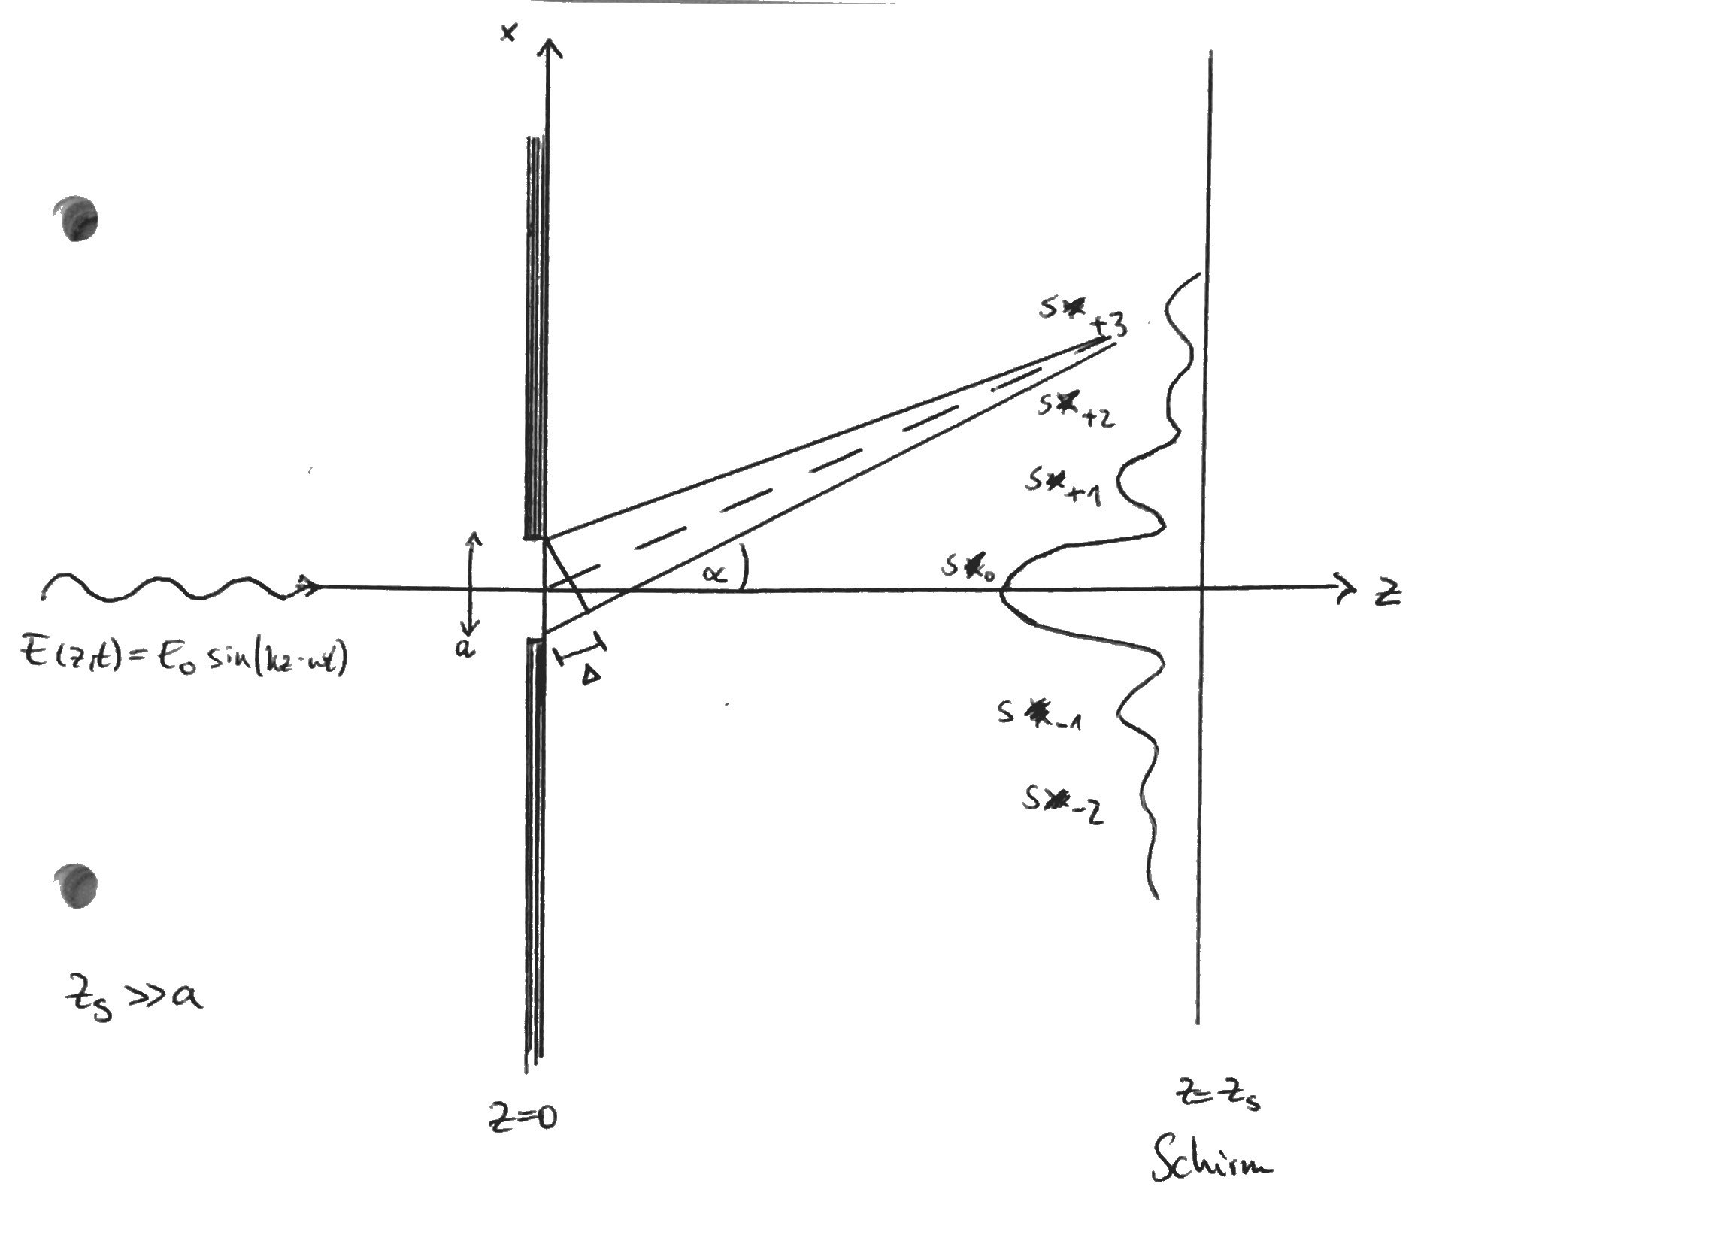
\includegraphics[scale=0.7]{einzelspalt.pdf}
\caption{Skizze mit allen relevanten Variablen für den Einzelspalt}
\end{figure}

\section{1-dim N-Spalt}
\end{document}